\begin{tikzpicture}
\begin{axis}[width=\marginparwidth+25pt,%
tick label style={font=\scriptsize},axis y line=middle,axis x line=middle,name=myplot,axis on top,%
%			xtick={-5,-4,-3,-2,-1,1,2,3,4,5},% 
%			extra x ticks={3.14,1.57},
%			extra x tick labels={$\pi$,$\pi/2$},
%			ytick={-1,-2,1,2},
			%minor y tick num=1,%extra y ticks={-5,-3,...,7},%
%			minor x tick num=4,
			ymin=-.1,ymax=3.5,%
			xmin=-1,xmax=11%
]

\addplot [{\colorone},domain=0:10,smooth,thick,samples=50] coordinates {(0,0)(0.016,0.1265)(0.032,0.1789)(0.048,0.2191)(0.064,0.253)(0.08,0.2828)(0.096,0.3098)(0.112,0.3347)(0.128,0.3578)(0.144,0.3795)(0.16,0.4)(0.176,0.4195)(0.192,0.4382)(0.208,0.4561)(0.224,0.4733)(0.24,0.4899)(0.256,0.506)(0.272,0.5215)(0.288,0.5367)(0.304,0.5514)(0.32,0.5657)(0.336,0.5797)(0.352,0.5933)(0.368,0.6066)(0.384,0.6197)(0.4,0.6325)(0.8,0.8944)(1.2,1.095)(1.6,1.265)(2.,1.414)(2.4,1.549)(2.8,1.673)(3.2,1.789)(3.6,1.897)(4.,2.)(4.4,2.098)(4.8,2.191)(5.2,2.28)(5.6,2.366)(6.,2.449)(6.4,2.53)(6.8,2.608)(7.2,2.683)(7.6,2.757)(8.,2.828)(8.4,2.898)(8.8,2.966)(9.2,3.033)(9.6,3.098)(10.,3.162)};
\addplot [{\colortwo},smooth,thick] coordinates {(0,0.5469)(0.2,0.6536)(0.4,0.7551)(0.6,0.8518)(0.8,0.944)(1.,1.032)(1.
2,1.116)(1.4,1.196)(1.6,1.273)(1.8,1.346)(2.,1.417)(2.2,1.485)(2.4,1.
55)(2.6,1.613)(2.8,1.673)(3.,1.732)(3.2,1.789)(3.4,1.844)(3.6,1.897)(
3.8,1.949)(4.,2.)(4.2,2.049)(4.4,2.098)(4.6,2.145)(4.8,2.191)(5.,2.
236)(5.2,2.28)(5.4,2.324)(5.6,2.366)(5.8,2.408)(6.,2.448)(6.2,2.488)(
6.4,2.527)(6.6,2.565)(6.8,2.602)(7.,2.637)(7.2,2.672)(7.4,2.705)(7.6,
2.737)(7.8,2.768)(8.,2.797)(8.2,2.824)(8.4,2.849)(8.6,2.873)(8.8,2.
894)(9.,2.913)(9.2,2.929)(9.4,2.942)(9.6,2.953)(9.8,2.96)(10.,2.964)};
%\addplot [{\colortwo!40},domain=-4:4,thick,smooth] {-x^4/2-x^3/6+x^2+x+2};

\draw (axis cs:8.,1) node {\begin{tikzpicture}
						\draw[thick,{\colorone}] (0,0)--(10pt,0) node [right,black] {\scriptsize $y= \sqrt x$};
						\draw[{\colortwo},thick] (0,-10pt)--(10pt,-10pt) node [right,black] {\scriptsize $y= p_4(x)$};
													\end{tikzpicture}};
%\draw (axis cs:-2,-2.75) node {\scriptsize $y=p_{13}(x)$};



\end{axis}

\node [right] at (myplot.right of origin) {\scriptsize $x$};
\node [above] at (myplot.above origin) {\scriptsize $y$};
%\node [below] at (myplot.below origin) {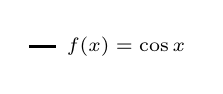
\begin{tikzpicture} \draw[thick,{\colorone}] (0,0)--(10pt,0) node [right,black] {\scriptsize $f(x)= \cos x$};\end{tikzpicture}};

\end{tikzpicture}




